%-------------------------------------------------------------------------------
\section{Methodology}
%-------------------------------------------------------------------------------
\begin{figure}[h]
\begin{center}
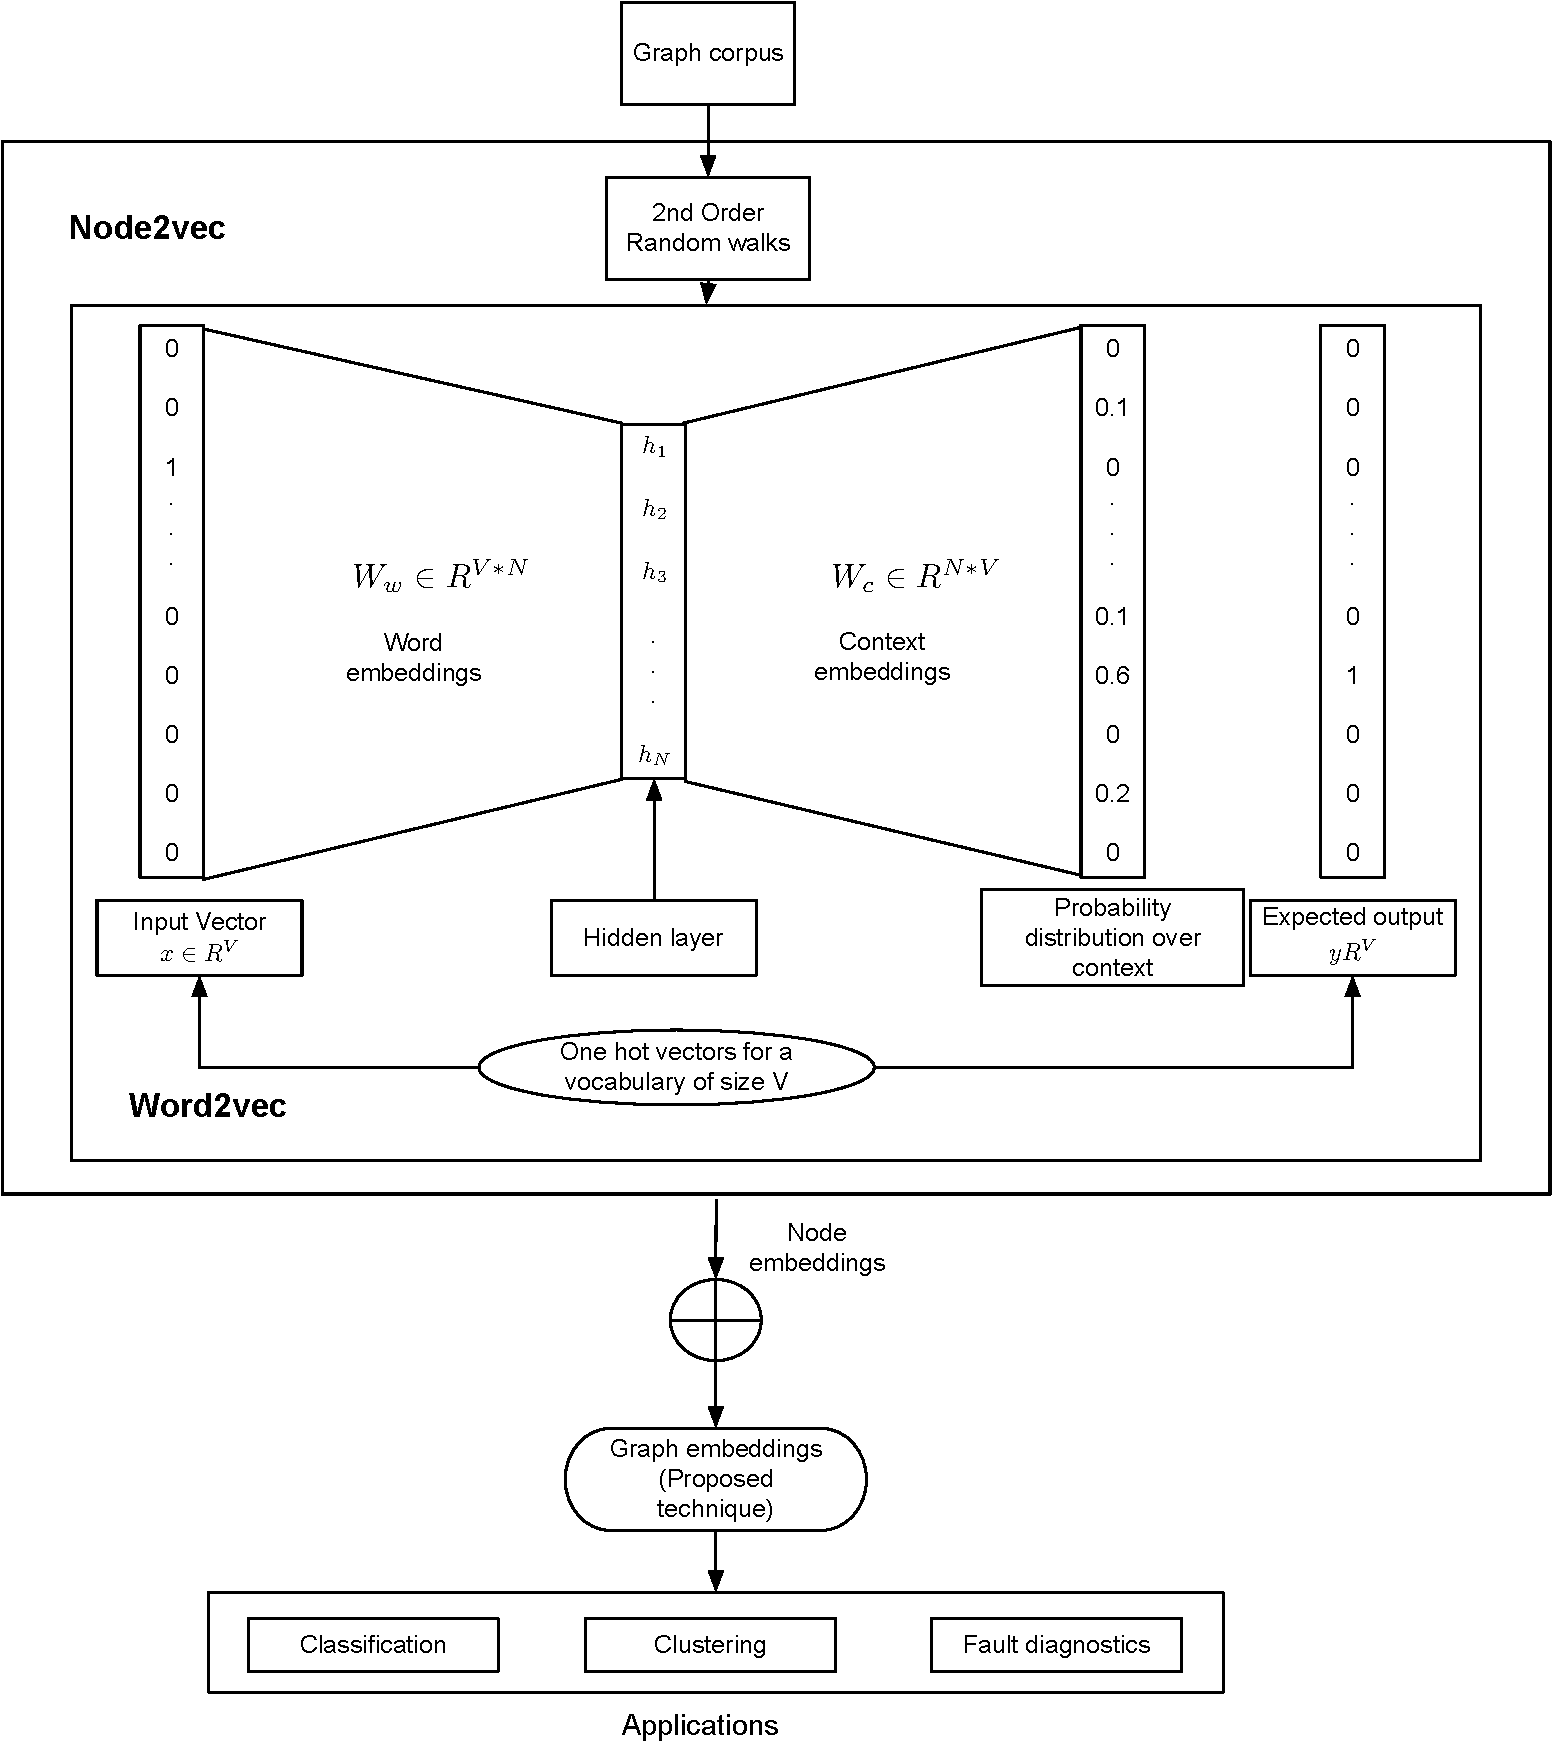
\includegraphics[width=0.4\textwidth, scale=0.25]{system_model.pdf}
\caption{System Model} 
\label{System_model}
\end{center}
\end{figure}

There are many possible representations to encode a graph as a representation. The choice of representation is usually driven by the downstream task to be performed. 

Our approach is to learn representations automatically from data i.e. graphs from traces of successful interactions. We compute our graph embedding as a composite of embeddings of nodes in the graph, as this is the approach commonly taken in previous work~\cite{corr_2017_abs-1709-05584}.
Of the various aggregator functions available, summation is simple and scalable. For precisely these reasons, it has been used in prior work~\cite{DBLP:journals/corr/DuvenaudMAGHAA15, DBLP:journals/corr/DaiDS16} to obtain subgraph embeddings. Intuitively, the resultant graph embedding is a linear combination of the component node embeddings. 
Grover et al.~\cite{corr18_GroverL16} describe node2vec, which obtains node embeddings for graphs analogous to word embeddings obtained for documents. To summarize, graph nodes are considered words and random walks in the graph generate sentences for us to train on. As a result, the node embeddings encode information about its structural neighborhood. We use node2vec to obtain component embeddings.  

For a graph G, the baseline representation R is vector of dimension D, where D is the the number of distinct services. Then, \newline
\begin{math}
Map(S_{1}) \in {0..D-1} \\
Map(S_{i}) \neq Map(S_{j}),\;  i \neq j,\; 1 \leq i,j \leq D \\
    Let\; m =\; Map(S_{i})\; \forall i \in {1..D} \\
    R[m] = 
    \begin{cases}
        1, S_{i} \in G \\
        0, S_{i} \notin G \\
    \end{cases}
\end{math}

In the next section, we describe how our approach compares vis-a-vis the baseline as well as initial results for each of the tasks in the figure.
